\documentclass[a4paper,11pt,titlepage]{scrartcl}
\usepackage[dutch]{babel}
\usepackage[T1]{fontenc}
\usepackage[utf8]{inputenc}
\usepackage{lmodern}
\usepackage{amssymb}
\usepackage{color}
\usepackage{graphicx}
\newcommand{\tab}{\hspace*{2em}}

\title{\huge\textbf{Excel++}}
\titlehead{\centering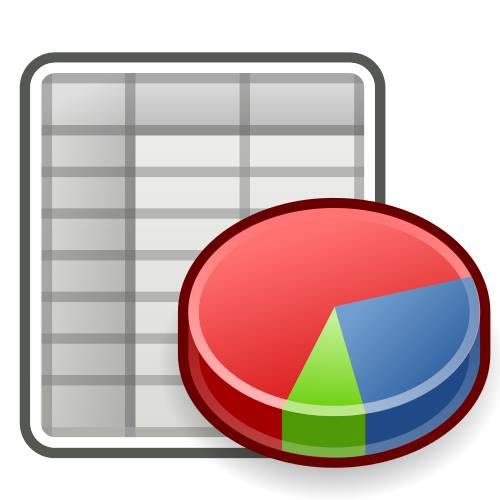
\includegraphics[width=6cm]{eindverslag.jpg}}
\author{\textbf{Team Awesome:}\\
		Bernd Kreynen 4331842\\
		Dave Grund 4291999\\
		Gerlof Fokkema 4257286\\
		Jente Hidskes 4335732\\
		Joris Lamers 4233042\\
		Skip Lentz 4334051\\
	   }

\begin{document}
\begin{titlepage}
\maketitle
\thispagestyle{empty} %geen page numbering op opening pagina
\end{titlepage}

\setcounter{tocdepth}{2}
\tableofcontents

\newpage\section{Algemeen: hoe het project is verlopen}
Het doel van dit project was het verbeteren van de kennis van Java en het opdoen van ervaring met werken in een team. De opzet was om een spreadsheet applicatie te maken voor een denkbeeldige klant, waarbij alles zo echt mogelijk moest gaan. Het begon met de vraag van de klant: \textit{''Maak een spreadsheet applicatie voor mij''} en daarmee was de opdracht geleverd. Er waren drie harde eisen: het inlezen en wegschrijven van een XML bestand, het maken van een grafische user interface (voortaan GUI genoemd) en het implementeren van vijfentwintig formules. Buiten deze eisen om, waren we vrij om te doen en laten wat wij wilden - mits de klant akkoord ging bij de wekelijkse bespreking. Dit liet dus heel veel over om zelf in te vullen; hoe wij dit hebben aangepakt leest u in dit verslag.\\

Van begin af aan was er in onze groep een duidelijke taakverdeling: de groep van zes is opgesplitst in tweetallen met ieder hun eigen taak. Zo werkte één tweetal aan de XML-reader en -writer en de formules, werkte een ander tweetal aan de parser voor de formules en de implementatie van Cellen en werkte het laatste tweetal aan de GUI. Doordat er zo’n duidelijke taakverdeling was, werd het hele project overzichtelijk en was het makkelijk om overleg te voeren. Er werd eerst overleg gepleegd binnen het tweetal en daarna over de conclusies van de andere tweetallen. Zo zijn eindeloze discussies en het tegelijkertijd implementeren van dezelfde feature voorkomen.\\

Helemaal in het begin, bij de eerste meeting, is er eerst gebrainstormed over een naam: Excel++. Vervolgens is er overleg gepleegd over wat voor features Excel++ moest hebben. Daarna is de taakverdeling gemaakt, onder andere gebaseerd op ervaring die sommige teamleden al hadden: Gerlof heeft al \textit{''real world''} ervaring met programmeren dus zou hij de formule parser en de implementatie van Cellen op zich nemen, omdat dit een kritiek onderdeel van elk spreadsheet programma is. Jente had al ervaring met het maken van GUIs (GTK+ toolkit op Linux), dus nam hij dit onderdeel voor zijn rekening. Tot slot had Joris al ervaring met XML bestanden, omdat hij naast student ook webdeveloper is. Hij zou dus de XML-reader en -writer en de formules maken.\\

De gemaakte planningen waren eenvouding: \textit{''het grondwerk voor feature X is nu gelegd, dus volgende week is dat op zijn minst basaal ge\"{i}mplementeerd''}. Zo zijn we iedere week bij elkaar gekomen om te kijken waar we waren op de SCRUM planning, wat er nog moest gebeuren op deze planning en welke features nu dan aan de beurt waren. Logischerwijs moest er met sommige features gewacht worden totdat andere waren ge\"{i}mplementeerd, maar dit was geen probleem. De hele groep hield zich aan de planning en er is nooit een periode geweest dat het ene tweetal op het andere moest wachten. Dit had tot gevolg dat iedereen op zijn eigen tempo door kon werken en dat steeds elke sprint zoals gepland doorlopen werd.\\

\newpage Overleg plegen gebeurde, naast de wekelijkse bijeenkomst, voornamelijk via Facebook. Hier hebben wij een speciale, private pagina op aangemaakt voor onze groep. Richting het einde van het kwartaal werd er ook gebruikt gemaakt van de Issues pagina op GitHub, maar deze diende voornamelijk als bugtracker en niet voor het overleggen over technische afwegingen. Er is voor Facebook gekozen omdat iedereen hier toch wel dagelijks even naar kijkt en dit bij bijvoorbeeld email niet het geval is. Als het GUI-team een nieuwe methode nodig had van de klasse Cell of een wijziging in het TableModel, was het erg fijn dat dit nog diezelfde middag gedaan kon worden. Via Facebook was dit mogelijk. Facebook bleek ook handig voor het terugkijken op eerder gemaakte beslissingen: alles is handig op chronologische volgorde terug te vinden, met de reacties van groepsleden erbij. Zoals gezegd is er ook gebruik gemaakt van de Issues pagina van GitHub als bugtracker. Deze pagina is erg handig voor het centraal bijhouden van bugs of nog missende features. Ook hier is enig overleg gepleegd, wat wel resulteerde tot twee plaatsen van overleg en dus soms wel enig zoekwerk naar de juiste informatie. Een leuke bijkomendheid van de Issues op GitHub is de drang die je hebt om het aantal geopende Issues zo laag mogelijk te houden: zo word je nog gemotiveerder om bugs te squashen!\\

Het gebruik van Git was niet alleen handig vanwege GitHub’s Issues pagina. Er is in onze groep veelvuldig gebruik gemaakt van branches, van Git’s rebase mogelijkheid en om simpelweg een commit te kunnen reverten. Tot twee keer toe was er een probleem met de master branch, maar mede dankzij de lokale kopieën zijn we altijd in staat geweest om dit op te lossen. De mogelijkheid om \textit{diff’s} van elke commit na te kijken is ook erg handig om te zien wat er precies is veranderd. Dit biedt de mogelijkheid om te zien of iets niet beter op een andere manier gedaan had kunnen worden. Er kan dus geconcludeerd worden dat het gebruik van versiebeheer ons zeker heeft geholpen.\\

\newpage\section{Ontwerpproces}
Gedurende het ontwerpproces zijn er verschillende momenten geweest waarop er belangrijke ontwerpbeslissingen genomen moesten worden. Naarmate het project vorderde bleek het dat sommige keuzes niet de juiste waren. In dit hoofdstuk zullen een aantal van deze afwegingen worden uitgelicht en besproken. Bij het nemen van beslissingen is er zoveel mogelijk rekening gehouden met voornamelijk de volgende aspecten:
\begin{itemize}
	\item platform onafhankelijkheid;
	\item beschikbaarheid van documentatie;
	\item performance en geheugengebruik;
	\item gemak van gebruik.
\end{itemize}

Van begin af aan was de doelstelling om Excel++ zo modulair mogelijk te laten zijn: componenten moesten eenvoudig vervangen of toegevoegd kunnen worden zonder dat er uitgebreide wijzigingen in de code nodig waren. Uiteraard had dit tot gevolg dat de Model View Controller gebruikt zou moeten worden. Hier wordt later op teruggekomen.

In het begin van het project dienden er gelijk twee belangrijke technologische afwegingen gemaakt te worden, namelijk welke libraries er gebruikt zouden worden voor het uitlezen en het wegschrijven van de XML bestanden en voor het weergeven van de GUI.\\

\subsection{De XML-reader en -writer}
De technologische afweging die hier gemaakt moest worden was welke API er gebruikt zou worden voor het uitlezen van XML bestanden: JAXP DOM of JAXP SAX. Van deze twee APIs, die beiden binnen de standaard API van Java zitten, zijn de voor- en nadelen onderzocht:
\begin{description}
	\item \textbf{JAXP DOM}
		\begin{description}
			\item[+] Makkelijk in gebruik omdat de hele XML als DOM in het geheugen staat;
			\item[+] Makkelijk in gebruik door \textit{''DOM traversal''};
			\item[+] Kan ook gebruikt worden voor het wegschrijven van XML bestanden;
			\item[-] Verbruikt meer geheugen omdat de hele XML als DOM in het geheugen staat;
			\item[-] Is minder snel en efficiënt dan een event based XML parser.
		\end{description}
	\item \textbf{JAXP SAX}
		\begin{description}
			\item[+] Sneller, vooral bij grote bestanden;
			\item[+] Verbruikt minder geheugen;
			\item[-] Lastiger te implementeren in verband met callbacks;
			\item[-] Kan niet gebruikt worden voor het wegschrijven van XML bestanden.
		\end{description}
\end{description}

De belangrijkste argumenten voor het gebruik van JAXP SAX zijn dus voornamelijk de snelheid en het geheugengebruik. Hiertegenover staan de belangrijkste argumenten voor het gebruik van JAXP DOM, namelijk het gebruiksgemak en het kunnen wegschrijven van bestanden met dezelfde library. Na het programmeren van een kleine testcase bleek het snelheidsverschil niet groot genoeg om te kiezen voor JAXP SAX en is er dus gekozen voor JAXP DOM, daar deze library nu de meeste voordelen overhoudt.

\subsection{De grafische toolkit}
De volgende technologische afweging die gemaakt moest worden was welke toolkit er gebruikt zou worden voor de GUI. Er waren vier gangbare keuzes: JavaFX, SWT, AWT en Swing. Hiervan is SWT gemaakt door de ontwikkelaars van Eclipse (ten behoeve van de Eclipse IDE) en de rest door de ontwikkelaars van Java. Ondanks dat JavaFX dus intern ontwikkeld is, werd het lang niet standaard meegeleverd bij de Java Development Kit: pas vanaf versie 7u45 is het beschikbaar. Op dit moment wordt Swing gezien als de standaard voor het programmeren van GUIs met Java. Swing bouwt tevens voort op AWT, dat hierdoor eigenlijk al door ons werd afgeschreven omdat het al een opvolger heeft.\\

Ook van al deze toolkits zijn de voor- en nadelen onderzocht, die hier onder kort worden samengevat:
\begin{description}
	\item Swing
		\begin{description}
			\item[+] Gedraagt zich op alle platformen vrijwel hetzelfde;
			\item[+] Wordt gezien als de standaard;
			\item[+] Er is uitgebreide documentatie, inclusief vele tutorials, beschikbaar;
			\item[+] Komt intuïtief over;
			\item[+] Maakt standaard gebruik van de Model View Controller;
			\item[-] Is niet thread-safe;
			\item[-] Swing componenten zijn over het algemeen langzamer dan die van AWT;
			\item[-] Native look and feel is niet echt native: er blijven kleine verschillen.
		\end{description}
	\item AWT
		\begin{description} 
			\item[-] Gedraagt zich niet helemaal hetzelfde op alle platformen;
			\item[-] Wordt tegenwoordig minder gebruikt dan Swing;
			\item[-] Kan als ''verouderd'' worden beschouwd, waarvan Swing de ''opvolger'' is;
			\item[-] Er is geen component om een tabel te maken;
			\item[-] Kan geen icons en tooltips weergeven.
		\end{description}
	\newpage\item SWT
		\begin{description}
			\item[+] Gebruikt native elementen waar mogelijk;
			\item[-] Gedraagt zich niet helemaal hetzelfde op alle platformen;
			\item[-] Komt weinig intuïtief over;
			\item[-] Wordt relatief minder gebruikt dan Swing;
			\item[-] Vereist native libraries voor elk Operating System.
		\end{description}
	\item JavaFX
		\begin{description}
			\item[+] Ziet er grafisch erg mooi uit;
			\item[-] Heeft een stijle leercurve;
			\item[-] Is nog redelijk nieuw en daarmee minder uitgebreid getest;
			\item[-] Wordt relatief minder gebruikt dan Swing.
		\end{description}
\end{description}

Omdat binnen onze groep alle drie de gangbare Operating Systems wordt gebruikt, is platform onafhankelijkheid een erg belangrijk argument geweest. Hierdoor zijn SWT en AWT afgevallen. JavaFX is nog relatief nieuw, wat tot gevolg heeft dat het weinig documentatie en voorbeelden heeft. Daarnaast heeft JavaFX ook een stevige leercurve. Swing's API komt intuïtief over en heeft veel documentatie en voorbeelden. Aangezien dit onze eerste ervaring met het programmeren van GUIs (al dan niet in Java) is, heeft dit een grote invloed op onze keuze gehad.\\

Om deze redenen is de conclusie getrokken dat geen van de alternatieven ons tijdens het ontwikkelen van Excel++ genoeg voordelen biedt om af te wijken van de standaard: Swing. Deze toolkit biedt gegarandeerd de mogelijkheid om te voldoen aan de Model View Controller: de Cellen kunnen in een TableModel worden gestopt, om vervolgens ingelezen te worden in de JTable van de GUI. Hoe deze TableModel geconstrueerd is, komt in de volgende paragraaf aan bod.\\

\newpage\subsection{De SpreadSheet TableModel}
Java biedt een standaard interface voor het modelleren van data voor tabellen. Er is besloten om van deze mogelijkheid gebruik te maken door het SpreadSheet model te baseren op de Java klasse AbstractTableModel. Op deze manier wordt het dynamisch updaten van de GUI automatisch geregeld door Java. Hierdoor hoeft er enkel rekening te worden gehouden met de manier waarop de data wordt opgeslagen en teruggegeven aan de JTable. In de SpreadSheet klasse wordt de data opgeslagen in een één-dimensionale HashMap. Dit is geïmplementeerd door een (x, y) coordinaat als volgt te vertalen naar een integer:
\begin{verbatim}
int index = x * totalRows + y;
\end{verbatim}

Door het gebruik van een HashMap is het ophalen van Cellen, dankzij hun index, zeer snel. Verder is het bij een HashMap mogelijk om bijvoorbeeld indices twee en vijf te vullen en indices één, drie en vier over te slaan. Hierdoor kan de HashMap minder Cellen bevatten dan dat er in de GUI getoond worden. Dit kan bij Arrays bijvoorbeeld niet. Dit komt de efficiëntie en het geheugengebruik ten goede.

\subsection{De plugin architectuur van de formules}
Een harde eis van het project is dat Excel++ op zijn minst vijfentwintig verschillende formules dient te ondersteunen. Bij het ontwikkelen van Excel++ is gestreefd naar een modulair programma en daarom is het wenselijk dat dit ook in de formules terug te vinden is: zij moeten op zichzelf staand toe kunnen worden gevoegd aan het programma. Andy Zaidman heeft tijdens één van de colleges geopperd om dit te doen middels een ''plugin architectuur''. De enige andere mogelijkheid om dit te implementeren is om de lijst van formules vantevoren vast te stellen. Dit betekent dat er ergens een lange lijst van formules bijbehouden moet worden die elke keer na het toevoegen van een formule bijgewerkt moet worden. Dit past uiteraard niet bij het streven naar een modulair programma, dus is er gekozen voor de ''plugin architectuur''.

Dit is in Excel++ geïmplementeerd door op basis van input van de gebruiker dynamisch een formule-klasse in te laden uit het package com.awesome.excelpp.math. Op deze manier hoeft er bij het toevoegen van een nieuwe formule enkel een nieuwe klasse aangemaakt te worden in deze package. Zo'n nieuwe klasse moet dan de abstracte klasse Formula \textit{extenden} en heeft zodanig naast een vaste structuur, ook een paar hulp-methodes tot zijn beschikking. Verder dient de naam van de klasse exact overeen te komen met de naam van de formule. Na het toevoegen van de nieuwe klasse is de formule automatisch beschikbaar in Excel++.

\newpage Het implementeren van deze structuur brengt een aantal problemen met zich mee:
\begin{itemize}
	\item het package com.awesome.excelpp.math mag geen subpackages bevatten;
	\item formules moeten allen dezelfde (lege) constructor bevatten;
	\item formules mogen geen output teruggeven of excepties opgooien die de parser niet verwacht;
	\item formules mogen geen System.exit(0) of ander onverwacht gedrag implementeren.
\end{itemize}
Omdat het grootste deel van deze problemen alleen speelt wanneer formules uit packages van derden toegevoegd worden is ervoor gekozen om met deze problemen geen rekening te houden.

\subsection{De overstap van de infix parser naar de shunting-yard parser}
De eerste versie van de formule parser evalueerde direct vanuit de gegeven wiskundige expressie. Deze expressie is gegeven in infix notatie: de notatie die de meeste mensen gewend zijn.\\

Het probleem, echter, was dat het implementeren van de wiskundige bewerkingsvolgorde lastig was: het resulteerde in code die methoden aanriep in methoden. Hierdoor was de code uiteindelijk lastig te begrijpen, dat automatisch ook het optimaliseren ervan en het opsporen van bugs moeilijker maakte.\\ Om die reden is de overstap gemaakt naar een ander soort parser, waarbij eerst de expressie wordt omgezet naar ''Poolse notatie'', welke ook wel postfix notatie wordt genoemd. Deze expressie is makkelijker en sneller te evalueren dan een expressie in de infix notatie. Het omzetten zelf is gedaan met behulp van het Shunting-yardalgoritme (rangeerstationalgoritme), uitgevonden door E.W. Dijkstra. Met het evalueren van de nieuw verkregen expressie hoeft er geen rekening meer te worden gehouden met de wiskundige bewerkingsvolgorde, behalve bij expressies tussen haakjes.\\

Ook is de overstap gemaakt naar het gebruiken van een state machine (eindigetoestandsautomaat) in plaats van regex patronen bij het omzetten naar Tokens. Het is bekend dat regex erg simpel te implementeren is, maar wel zeer traag in uitvoer. In het begin is er daarom regex gebruikt en zou er overgestapt worden op een andere manier van \textit{''tokenizen''} als er tijd genoeg voor was.

\newpage\subsection{De overstap van het String datatype naar het Cell datatype}
Voor het representeren van spreadsheet data is er een klasse SpreadSheet ontwikkeld, gebaseerd op het AbstractTableModel van Java Swing. Deze klasse houdt, zoals vermeld, referenties naar alle Cell objecten bij in een HashMap en biedt de GUI de mogelijkheid om waarden op te vragen. De standaard AbstractTableModel API biedt echter enkel methoden zodat er omgegaan kan worden met het datatype Object.\\

De JTable API biedt de mogelijkheid om een CellRenderer en een CellEditor in te stellen, echter wordt er standaard alleen een CellRenderer en een CellEditor voor het omgaan met Strings en booleans meegeleverd. Doordat de JTable en het AbstractTableModel enkel met Objects, Strings en booleans om kunnen gaan is er dus geen mogelijkheid om opmaak in te stellen voor Cellen in de datarepresentatie.\\

Daarom is er gekozen om een eigen AwesomeCellRenderer en AwesomeCellEditor te ontwikkelen en om binnen het AbstractTableModel enkel gebruik te maken van Cell objecten. Op deze manier kunnen er in de GUI makkelijk Cell objecten worden aangevraagd en is van de Cell objecten zelf eenvoudig de opmaak te wijzigen. Omdat de Cell hierdoor zelf verantwoordelijk is voor het opslaan van zijn eigen opmaak blijft het correct wegschrijven van Cell eigenschappen, zoals inhoud en opmaak, bovendien eenvoudig.

\subsection{De overstap van Double naar Object in de formule parser}
In het begin van het project is ervoor gekozen om te streven naar een goede basis voor de applicatie. Dit had tot gevolg dat er wel een aantal van de verplichte formules geïmplementeerd waren, maar nog lang niet allemaal. Daardoor is vrij laat naar voren gekomen dat de formule parser niet alleen het inlezen van Doubles moest ondersteunen, maar ook ook het inlezen van Strings. Een aantal formules kunnen namelijk ook Strings als argument meegegeven krijgen of kunnen String returnen; bijvoorbeeld de formule Lower. Daarnaast wilden we, naast de verplichte functionaliteit, ook kunnen omgaan met Booleans en Integers. Om dit probleem op te lossen is er besloten om de formule parser te baseren op het Object datatype in plaats van op het datatype Double. Hierdoor kan de parser nu Strings en Doubles genereren en opslaan als een Object. De formule beslist later zelf met behulp van \textit{instanceof} of zijn argumenten een String, een Boolean, een Integer of een Double zijn. Wanneer de argumenten van de formule niet zijn zoals verwacht, dan wordt er een exceptie opgegooid.

\newpage\subsection{De modulaire structuur van de Writer-klasse}
Omdat het AbstractTableModel SpreadSheet de data representatie van de spreadsheet bevat, is er in eerste instantie voor gekozen om ook het wegschrijven naar een XML bestand onderdeel te maken van de klasse SpreadSheet. Dit paste echter niet goed in het streven naar een zo modulair mogelijke applicatie. Bovendien zou dit het toevoegen van ondersteuning voor andere bestandstypen lastig maken. Dit is de reden geweest om het wegschrijven van XML bestanden ook modulair te maken. Dit heeft tot gevolg gehad dat de klasse SpreadSheet nu communiceert met een Writer interface. De XML Writer implementeert vervolgens deze interface. Als er eventueel extra Writers toegevoegd gaan worden, hoeven deze nu alleen de Writer interface te implementeren. Als demonstratie van deze Writer interface is de extra Writer SysOutWriter toegevoegd en indien mogelijk wordt voor het einde van het project nog ondersteuning voor CSV bestanden geïmplementeerd.

\subsection{De grafieken}
Er is pas aan het einde gekeken naar grafieken, omdat dit een uitbreiding was en eerst de basisfunctionaliteit zo goed als geïmplementeerd moest zijn. Dit had tot gevolg dat er weinig tijd was om onderzoek te doen naar de verschillende libraries, dus was er één nodig die makkelijk in gebruik was om alles snel geïmplementeerd te krijgen. Een simpele library zorgt ook voor een kleinere kans op bugs van onze kant uit. Zowel JFreeChart als BIRT bevatten alle functionaliteit die Excel++ nodig zou hebben, maar JFreeChart bleek makkelijker in gebruik. Bovendien heeft een standaard grafiek van deze library veel meer opties: zonder hiervoor code te moeten schrijven is er al een optie menu, met opties als \textit{save as PNG} en een mogelijkheid tot in- en uitzoomen. Daarom is er dus gekozen voor JFreeChart om grafieken te implementeren.

\subsection{Observer/Observable}
Tijdens het implementeren van de basis van het project is er zoveel mogelijk rekening gehouden met efficiëntie en het gebruik van resources. Voor het ontwikkelen van de GUI is hier echter minder rekening mee gehouden. De oorzaak hiervan ligt grotendeels bij het feit dat het begrip van JTable en AbstractTableModel aan het begin van het project nog niet voldoende was om hier goed over na te kunnen denken.\\

Tijdens het project is hier echter goed genoeg kennis mee gemaakt. Een belangrijke verandering die dit teweeg heeft gebracht is het implementeren van Observers en Observables. Gedurende het project werd de GUI namelijk geüpdatet door bij elke setValue in het SpreadSheet model de methode fireTableDataChanged aan te roepen, wat tot gevolg heeft dat de hele tabel opnieuw gerenderd dient te worden. Door het SpreadSheet data model een Observer te maken en door de Cell objecten een Observer en een Observable te maken zijn dynamische updates van de GUI mogelijk gemaakt, zonder iedere keer de hele GUI te moeten renderen.

\newpage Hier zaten helaas nog wat haken en ogen aan vast, aangezien Observers volgens hun isEquals methode niet gelijk mogen zijn aan andere Observers. Dit heeft tot gevolg gehad dat een flink deel van de Observer functionaliteit zelf geïmplementeerd moest worden. Een ander lastig punt bij het implementeren van Observers / Observables was dat het updaten van de content van het model op verschillende manieren gedaan kan worden. Hierdoor moet op verschillende plaatsen rekening gehouden worden met mogelijke wijzigingen. Als het updaten van het model in één klasse gecentraliseerd wordt, dan is het veel makkelijker om updates van de GUI te implementeren. Hier wordt verder op ingegaan bij de verbeterpunten in hoofdstuk drie.

\subsection{Het nut van het UML-diagram}
Een aantal van de genomen beslissingen hebben een grote impact gehad op het ontwerp van het programma. Vooral ook de beslissingen die later genomen waren, nadat er meer kennis opgedaan was, hebben af en toe flinke gevolgen gehad. Twee voorbeelden hiervan zijn het omschakelen van String naar Cell objecten in het spreadsheet model en het omschakelen van Doubles naar Objects in de formule parser. Tijdens deze beslissingen heeft de UML geholpen om het overzicht op het ontwerp van het programma te behouden. Dankzij de UML was snel inzichtelijk wat voor impact dit soort wijzigingen op het programma gingen hebben en waar er tegen problemen aangelopen zou worden. Verder is het dankzij de UML ook makkelijk voor een teamlid om uit te leggen aan de groep waar hij precies aan werkt.\\

Een probleem waar wel tegenaan gelopen is, is dat het updaten van de UML niet altijd even frequent gedaan werd. Dit was echter geen probleem, omdat door onze taakverdeling voor iedereen zijn taak duidelijk was en de globale structuur van Excel++ wel altijd overeen kwam met die van het UML-diagram. Tevens kon er, als dit nodig was, via Facebook snel met verschillende mensen worden overlegd als iets niet duidelijk was or als er een nieuwe methode nodig was. Tot slot werd er wel voor gezorgd dat de structuur na ingrijpende wijzigingen weer klopte.

\newpage\section{Verbeterpunten}
Dit hoofdstuk behandelt twee verschillende onderwerpen: verbeterpunten in Excel++ en verbeterpunten voor het proces.\\

\subsection{Verbeterpunten in Excel++}
Ondanks dat we zeer te spreken zijn over het eindresultaat, zijn er op sommige aspecten nog wel verbeteringen door te voeren. Deze zullen hier kort worden uitgelicht.\\

Het eerste verbeterpunt zijn de resources die Excel++ in beslag neemt als het wordt uitgevoerd. Bij de formule parser is hier wel uitvoerig op gelet, maar de overige delen hebben meer de focus gelegd op features en op bugvrij zijn. Hoewel het, waar het kon, voor de minst resource-hungry optie is gekozen, denken wij dat hier nog wel wat winst te behalen valt; voornamelijk in de GUI zal dat het geval zijn.\\

Ook zouden de JUnit testen voor sommige formules wat uitgebreid kunnen worden. De formules waren aan het einde een probleem (zie \textbf{Planning} hieronder), waardoor sommige formules minder uitgebreid zijn getest.\\

Een ander verbeterpunt is het verbeteren van type checking tijdens het parsen van formules. Voor de standaard wiskundige operaties optellen, aftrekken, vermenigvuldigen en delen (+, -, * en /) wordt type checking in de parser gedaan. Voor alle andere formules, zoals Sum en Subtract, wordt type checking in de formule zelf gedaan voor meer flexibiliteit. Type checking in de parser is veel complexer en bovendien niet helemaal juist geïmplementeerd op dit moment. Door de wiskundige operaties zo te herschrijven dat ze gebruik maken van hun overeenkomende formules (dus + wordt Sum, - wordt Subtract et cetera) kan code duplicatie voorkomen worden en kan er makkelijker gegarandeerd worden dat de parser juist omgaat met foute of onverwachte invoer. De voornaamste reden dat dit nog niet geïmplementeerd is heeft te maken met het te laat wisselen naar een parser die werkt met het Object datatype.\\

Verder zijn gedurende het project de grenzen tussen een aantal klassen enigszins vervaagd, waardoor een aantal klassen niet meer zo flexibel zijn als ooit bedoeld. Een voorbeeld hiervan is dat de GUI tijdens het wijzigen van de content van een Cell geen interactie meer heeft met het SpreadSheet model. In plaats daarvan wordt de content direct in het Cell object gewijzigd. Dit heeft onder andere als gevolg dat het vrij lastig was om de GUI dynamisch te updaten met behulp van het Model View Controller model, omdat de Cell de SpreadSheet eerst moet laten weten dat deze gewijzigd is. Voor dit specifieke voorbeeld zou het wenselijk zijn om alle set-methoden uit de klasse Cell te verhuizen naar de SpreadSheet klasse. Op deze manier is de SpreadSheet model klasse weer volledig verantwoordelijk voor het bijhouden van wijzigingen en het updaten van de GUI.\newpage Een andere aanpak zou zijn om de GUI enkel toe te staan volledig opgemaakte cellen aan te laten maken via de Constructor van Cell en helemaal geen set-methoden toe te staan in de Cell-klasse zelf. De GUI-klasse kan dan vervolgens de SpreadSheet updaten met een volledig opgemaakte Cell. Ook bij deze aanpak wordt de SpreadSheet weer verantwoordelijk voor het bijhouden van wijzigingen en het doorgeven van updates.\\

Zoals in hoofdstuk twee vermeld is, zit er nog een veiligheidsrisico in de ''plugin architectuur'' van de formules. Het is vrij simpel om Excel++ ongewenste dingen te laten doen, omdat er niet gecontroleerd wordt welke code er precies in een formule-klasse zit alvorens deze uit te voeren. Er is nog geen oplossing bij ons bekend voor dit probleem.\\

Tot slot zijn er nog twee openstaande bugs op die Issues pagina van GitHub:
\begin{itemize}
	\item[1] er kan geen letterlijke '=' in een Cell worden getypt. Dit komt doordat de Cell, zodra er een '=' wordt getypt, automatisch de formule parser aanroept. Op zijn beurt, gooit de parser de '=' weg en probeert dan een lege expressie te evalueren. Dit resulteert in een lege Cell.
	\item[2] de Observer/Observable resulteert nog in een infinite loop bij \textit{Cell recursion}: als Cell A1 refereert naar Cell A2 en A2 refereert naar A1, dan wordt Cell A1 roodgekleurd vanwege een \textit{\#REFINV} (Invalid reference). Op zijn beurt, zou A2 dan ook rood moeten worden gekleurd. Dit triggert dan weer een repaint van A1... et cetera. Om dit te voorkomen, luistert A1 niet naar A2 en wordt deze dus pas weer wit (''gerepareerd'') als er in deze cel wordt geklikt.
\end{itemize}

\newpage\subsection{Verbeterpunten in het proces}
Tijdens het project waren er, hoewel het over het algemeen goed verlopen is, een aantal kleine problemen. In dit deel zullen deze besproken worden en wordt er, waar mogelijk, een suggestie voor verbetering gegeven. De grootste problemen waar verbetering zich nog toelaat zijn de volgende:
\begin{itemize}
	\item De planning;
	\item De deelopdrachten toewijzen (wie doet wat);
	\item Versiebeheer.
\end{itemize}

\subsubsection{Planning}
Hoewel we ons in het begin sterk aan onze SCRUM planning hielden en deze ook elke week updateten, nam dit patroon af naarmate het einde van ons project naderde. Vooral aan het einde hebben we de SCRUM planning in onze Google Drive map gelaten voor wat het was en hielden we voor een zeer korte periode alles bij in ons hoofd. Omdat dit niet werkte zijn we de Issues pagina op GitHub gaan gebruiken voor zowel bugs als \textit{todo's}. Hoewel deze aanpak wel liet zien wat er nog gedaan moest worden, gaf het geen overzicht van waar we ons binnen het verhelpen van de verschillende \textit{issues} bevonden. Bovendien gaf het ook niet aan wie deze \textit{issues} moest oplossen of implementeren (ondanks dat dit wel kan in GitHub), maar hierover later meer.\\

Alle hierboven genoemde nadelen van GitHub's Issues pagina doet een SCRUM planning wel; deze heeft namelijk vier kolommen, die aangeven in welke staat (TODO, IN PROGRESS, TESTING of DONE) de specifieke opdracht zich bevindt en wie er aan werkt. Nu was het wel een project op een kleinere schaal dan ''echte'' projecten dus konden we ons dit permitteren, maar we kunnen ons voorstellen dat als we bij een grootschalig project alles met de Issues pagina van GitHub bijhouden, dat een stuk lastiger verloopt.

Tot slot waren Dave en Joris te langzaam met het implementeren van de formules. Dit is geen schuldverwijzing naar Joris en Dave, want ook de rest is hier de fout in gegaan: zij hadden hier beter op moeten letten en al eerder moeten bijspringen. Het gevolg van het niet op tijd maken van de formules was dat er te laat feedback kwam op de mogelijkheden van de parser en daarom is deze een aantal keer flink bijgewerkt vlak voor de deadline. Eén van deze wijzigingen is de overstap van String objecten naar objecten van het type Object. Er zijn ook dingen die uiteindelijk niet meer geïmplementeerd zijn in de parser, zoals het doorgeven van niet-gequote booleans en Strings zonder aanhalingstekens (mits deze geen spaties bevatten). Nog belangrijker is dat de hele formule parser eigenlijk anders opgebouwd had moeten worden, als er vantevoren al naar de benodigdheden van de formules was gekeken. Uiteindelijk heeft de rest van het team het werk overgenomen om alle formules op tijd klaar en getest te krijgen. Dit is jammer en had niet gehoeven.

\subsubsection{Deelopdrachten toewijzen}
Dit probleem is eigenlijk een gevolg van het hiervoor beschreven probleem met de planning: aangezien we de SCRUM planning niet altijd bijhielden, wisten sommigen niet wat ze moesten doen op bepaalde momenten. We hadden gelukkig wel een wekelijkse vergadering, maar in de tijd tussen deze vergaderingen was dit probleem af en toe aanwezig. Er deden zich situaties voor waarbij er opeens veel functies waren ge\"{i}mplementeerd, zonder dat iemand überhaupt wist dat deze op de planning stonden. De oplossing voor dit probleem is dezelfde als de oplossing voor het hiervoor beschreven probleem: de SCRUM planning bijhouden.

\subsubsection{Git}
Behalve Jente en Gerlof, hadden we in het begin van het project geen of een beetje ervaring met Git en GitHub. Hoewel we tijdens dit project veel geleerd hebben over Git, is er natuurlijk veel te verbeteren op dit vlak, daar Git een enorm uitgebreide feature-set heeft. De verbeterpunten zijn niet zozeer dat we meer moeten \textit{''committen''} (al hebben we wel geleerd dat veel en vaak kleine commits doen de juiste aanpak is) of dat de beschrijvingen van commits beter moeten worden geformuleerd (\textit{''Changes''} laat erg veel ter verbeelding over): het heeft meer te maken met de verschillende functies van Git en het gebruiken van die functies. Zo is tot twee keer toe de master branch ''kapot'' gegaan en waren mensen soms in de war met branches en geweigerde pushes. Gelukkig konden Jente en Gerlof problemen met Git en GitHub vaak oplossen, maar hoe dit precies in zijn gang ging begrijpt de rest nog niet. Het zijn juist die dingen die Gerlof en Jente altijd oplosten die zij nog moeten leren.

\subsection{Individuele feedback}
\subsubsection{Bernd Kreynen}
Binnen het team heb ik voornamelijk, samen met Jente, aan de GUI van ons programma gewerkt. Ik had hier nog geen ervaring mee dus het was wel even wennen aangezien het wel wat anders is dan iets anders in Java programmeren. Hierdoor duurde het voor mij in het begin vaak ook vrij lang om eigenlijk vrij simpele functies te implementeren en heb ik ook soms, achteraf gezien, niet erg nette code geschreven. Daarbovenop kwam dan nog dat ik ook nog nooit GitHub had gebruikt dus daardoor kreeg ik ook soms wel onnodige vertraging. Gelukkig begon mijn kennis over Swing naarmate het project vorderde te groeien en ik heb dus ook het gevoel dat ik veel heb bijgeleerd.\\
De samenwerking binnen het team ging vrij vlot, wanneer er problemen waren was het makkelijk om even een berichtje op de Facebookpagina te plaatsen of om een Issue aan te maken op GitHub en hier kwamen dan altijd vrij snel reacties op. De takenverdeling was soms niet echt optimaal, het gebeurde wel eens dat het niet echt duidelijk was waar je nog aan kon werken of waar al aan gewerkt werd. Dit kwam voornamelijk omdat we niet altijd de SCRUM planning goed bijhielden. Gelukkig viel het meestal nog wel goed mee.
\subsubsection{Dave Grund}
Het geheel van het project liep goed binnen het team. Hieraan heeft iedereen op zijn eigen manier bijgedragen met zijn sterke en zwakke punten. In mijn geval was mijn zwakke punt dat de hoeveelheid werk die ik verzette achter bleef bij dat van de rest. Zij hadden vaak al meer gedaan en dan moest ik nog wat afmaken. Voor het volgende project zou ik zeker in het begin meer tijd moeten maken en sneller starten. Wat ik wel goed deed was me mengen in de gesprekken en het bijblijven van wat er moest gebeuren. Op bijna elk moment wist ik ook waar anderen aan bezig waren en kon ik met Joris en mijn deel daar op inspelen. De formules die Joris en ik deden gingen ook wat trager dan verwacht. Dit was omdat er in de opzet van het implementeren van deze formules nog wat moeilijkheden zaten. Dit was echter wel goed op te lossen en we hebben ze uiteindelijk op goede wijze weten te implementeren. Het verloop ging dus niet altijd even snel, maar wel goed. Er waren geen conflicten en de communicatie ging zonder moeilijkheden. Dit zie ik ook als een sterk punt van het team. Snelle en duidelijke communicatie maakten het veel makkelijker om het project tot een goed einde te brengen.
\subsubsection{Gerlof Fokkema}
Tijdens het project heb ik voornamelijk samengewerkt met Skip aan onze data models (SpreadSheet en Cell) en aan onze Parser. Daarnaast heb ik af en toe ook Jente ondersteund bij issues in de GUI. De samenwerking met Skip en Jente verliep prettig, aangezien Skip, Jente en ik allen plezier hadden in het verzinnen van oplossing voor het programmeerproject. Hierdoor was het, voornamelijk gedurende de opstartfase, erg makkelijk om het vereiste aantal uren te maken om op schema te blijven volgens de SCRUM planning.\\

Een van mijn sterke punten tijdens het project is geweest dat ik vrijwel altijd zicht had op waar iedereen mee bezig was. Daardoor had ik altijd overzicht op het programma als geheel. Een van mijn zwakkere punten komt hier dan ook direct uit voort: sommige design overwegingen heb ik zonder voldoende overleg doorgevoerd in ons project. Wel heb ik altijd geprobeerd om feedback te krijgen op dergelijke beslissingen en om ze toe te lichten via onze groepspagina op Facebook.\\

Tegen de slotfase van het project liepen er een aantal dingen mis. Volgens de SCRUM planning zouden voornamelijk Dave en Joris zich bezig houden met het implementeren van formules. De rest van het team heeft daardoor niet of nauwelijks naar formules gekeken. Aan het einde van het project bleek er echter nog veel werk verzet te moeten worden. Dit zorgde ervoor dat er op het laatste moment nog heel veel issues in de formule parser naar voren kwamen. Sommige van deze issues bleken te groot om op te lossen in de parser zoals deze nu is en vereisen eigenlijk een nieuw design. Door al deze nieuwe issues en doordat niet ieder teamlid even gemotiveerd was wist ik me tijdens de slotfase af en toe geen raad meer met alle dingen die er tegelijk moesten gebeuren.
\subsubsection{Jente Hidskes}
Mijn taak binnen het team was het maken van de GUI, wat ik samen deed met Bernd. Ik werkte graag aan de GUI, omdat ik al ervaring heb hiermee en dit voor mij dus het meest voor de hand lag om te doen. Ik wilde echter ook wel dingen leren en daarom heb ik me met van alles en nog wat bemoeid om overal iets van mee te krijgen. Dit had als resultaat dat ik samen met Gerlof het overzicht op het hele project had. Gerlof en ik hadden ook allebei al ervaring met Git en dus hielden wij samen de repository bij.\\
Een van mijn sterkere punten binnen het project was het verdelen van de taken en het bijhouden van de voortgang van het project. Een zwakker punt was wellicht dat ik hier een beetje in door schoot en te veel achter iedereen aan zat, maar ik heb hier geen klachten over ontvangen dus dit kan ik niet met zekerheid zeggen. Een tweede zwakker punt van mij was dat ik de SCRUM planningen begon te negeren en de Issues pagina op GitHub begon te gebruiken. Blijkbaar vond niet iedereen dit een fijne aanpak en ontstond er hierdoor wat verwarring. Conflicten met andere teamleden heb ik niet gehad.
\subsubsection{Joris Lamers}
Het mooiste van dit project vond ik om de werkelijke effectiviteit te ervaren van een SCRUM planning. Korte deadlines om een groter geheel in fases op te bouwen en na iedere deadline het gevoel dat er echt iets bereikt is. Het opdelen van het werk in kleine sub projecten ging ook beter dan gedacht. Iedereen was gefocusseerd op zijn deel en heeft zijn best gedaan zijn deel zo goed mogelijk uit te voeren. Dit geldt ook voor mij als ik kijk naar mijn inzet voor het project. Het was leuk om aan een kleiner deel te werken en dit meer in detail uit te kunnen werken. Alle functionaliteit die ik wilde heb ik toe kunnen voegen en zelfs meer. Ik heb mij niet al te veel met alle aspecten bezig gehouden, maar vooral gericht op mijn uit te voeren deel. Omdat heel de groep een deze gescheiden werkmentaliteit deelde, werkte dit naar mijn idee goed. Door het focussen op slechts een deel is het overzichtsplaatje wel lastiger. Ik weet hoe heel het project opgebouwd is, maar niet alles zo gedetailleerd. De onderlinge samenwerking was ik heel blij mee. Er is goed overlegd en gediscussieerd. Mede hierdoor en een strakke planning hebben we, naar mijn idee, meer kunnen doen dan we hadden verwacht. Een verbeterpunt voor mijzelf is mogelijk beter overzicht proberen te houden.
\newpage\subsubsection{Skip Lentz}
Ik heb het gevoel dat mijn positie binnen het team goed verliep; ik kon vaak mijn inbreng kwijt bij de anderen, brainstormen over idee\"{e}n, en oplossingen geven bij problemen. Dit deed ik vooral samen met Gerlof, aangezien hij mijn partner was in ons ''subteam''.
Een van de negatieve punten van mezelf is dat ik onvoldoende up-to-date was met wat er aan de hand was. Ik deed echter wel mijn best om, als er opeens iets nieuws was ge\"{i}mplementeerd, rond te vragen over hoe het allemaal zat. Dit was bijvoorbeeld het geval bij de eerste versie van onze Parser; deze was er opeens en ik was me daarvan te laat bewust. Op dat moment had ik echter wel spoedig gevraagd of Gerlof dit misschien kon uitleggen. Dit zie ik dus als \'{e}\'{e}n van mijn positieve punten.
Ons subteam hield zich vooral bezig met de Parser en het SpreadSheet/Cel model. Mijn kennis over de GUI is daarom vrij gelimiteerd, omdat ik me daar minder mee bezig heb gehouden. Dit had als gevolg dat wanneer daarover werd gesproken ik niet echt een inbreng kon geven wat betreft de GUI (negatief) zoals ik dat wel kon bij de Parser en het Spreadsheet/Cel model (positief).
Al met al is het wel vlot verlopen, met name met de tweede versie van onze Parser waarbij ik veel code heb kunnen bijdragen, in tegensteling tot de eerste versie van de Parser.
\end{document}
